%%%%%%%%%%%%%%%%%%%%%%%%%%%%
\section{Methods}\label{sec:Methods}
%%%%%%%%%%%%%%%%%%%%%%%%%%%%



%%%%%%%%%%%%%%%%%%%%%%%%%%%%
\subsection{Pink elephants}
%%%%%%%%%%%%%%%%%%%%%%%%%%%%

Pink elephants are generally orange, but they can be blue instead. There are several different species:
\begin{itemize}
\item The \emph{Blue Pink Elephant}, recognisable by its green colour.
\item The \underline{Checkerboard Eared Pink Elephant}, which can be recognised by its ears in the shape of a chess board.
\item The \textbf{Happy Pink Elephant}, which loves dancing.
\end{itemize}
All of these species are extinct.

\subsection{Chickens}
Chickens are not elephants. Generalising this principle, we get
\begin{equation}
	P_{Chicken} = (p - a)(p - b)(p - c) ... (p - z)P_{Elephant},
	\label{eq:Equation1}
\end{equation}
where $P_{Chicken}$ stands for the population of cows in The Netherlands. Thus, \autoref{eq:Equation1} does not have any implications for the population density of poisonous rubber duckies in Nigeria, since correlation does not imply causation. $\mathbf{QED}$.

% Normally, LaTeX just jumps to a new page itself, when it deems this necessary. But if you want to manipulate its decisions, use this command:
\newpage 



%%%%%%%%%%%%%%%%%%%%%%%%%%%%
\subsection{Hippopotamus}
%%%%%%%%%%%%%%%%%%%%%%%%%%%%
It was proven by C. Rocodile \cite{Rocodile2014} that pink elephants have absolutely nothing to do with hippopotamuses. \autoref{fig:Elephant} is not a picture of a hippopotamus:
\begin{figure}[h]
	\centering
	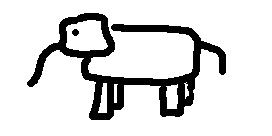
\includegraphics[width=150pt]{ElephantSimple}
	\caption{Not a hippo.}
	\label{fig:Elephant}
\end{figure}

\subsubsection{Hippopotamidae and math}
Hippopotami amphibii luuuv complicated looking math equations. The following is an example of an equation that a hippo notoriously solved by taking the Fourier Transform twice\footnote{...and swallowing another banana....}, after which he retired:
\begin{equation}
	\sum_{\substack{ 1 < i \leq \infty \\ j \neq i}}^{\reals}  \frac{\partial}{\partial \xi} \oint \mathcal{A + B} \, \diag \begin{pmatrix} 1 & 2 & 3 \\  4 & 5 & 6 \end{pmatrix} = \left(	x \frac{e^{2 \pi i \omega}}{r^2}	\right)^2.
\end{equation}
The relation of hyppopotamidae and numbers sets is as follows: $h \in \integers \in \reals$.